\begin{frame}{3.2 기둥}

\textbf{3.2.1 일반사항}

이 절은 축력이 예상축항복강도 $P_{ye}$의 10\%를 초과하는 기둥 부재에 적용한다. 

\begin{block}{ASCE 41-17 9.4.2.3.2 Columns}
	The strength of structural steel components under axial and flexural actions with a calculated axial load exceeding 10\% of the axial yield capacity, $P_{ye}$, shall be calculated in accordance with this section.
\end{block}

\begin{block}{AISC 342-XX (Draft) C3.1 General}
	This section shall apply to a member when the axial force (compression or tension) in the member equals or exceeds 10\% of $P_{CE}$ or $T_{CE}$ (...).
\end{block}
\textbf{3.2.2 기둥의 강성}

3.2.2.1 선형동적절차

선형동적절차를 위한 기둥의 강성은 구조역학 원칙에 기반하여 $\ulcorner$건축물 강구조 설계기준 (KDS 41 31 00:2019)$\lrcorner$에 따라 산정한다. 

\end{frame}


\begin{frame}{3.2 기둥}

	\textbf{3.2.2 기둥의 강성}

3.2.2.2 비선형정적절차

\begin{enumerate}
	\item[(1)] 기둥 부재의 탄성구간 강성은 3.2.2.1에 따라 산정한다. 
	\item[(2)] 기둥 부재의 축력 $P$가 예상축항복강도 $P_{ye}$의 50\%를 초과하는 경우, 탄성부재의 휨강성 $EI_c$는 $\ulcorner$강구조 골조의 안정성 설계기준 (KDS 14 31 15:2017)$\lrcorner$에 따른 강성저감계수 $\tau_b$를 적용하여 수정한다. 
	\[\tau_b = \begin{dcases}1.0 & \vert P\vert \leq 0.5 P_{ye} \\ 4\vert P\vert/P_{ye}(1 - \vert P\vert/P_{ye}) & \vert P\vert > 0.5 P_{ye}\end{dcases}\]
	\noindent 여기서 $P$는 하중조합으로 구해진 소요강도(압축 및 인장)이고, $P_{ye}$는 축항복강도($=F_{ye}A_s$)이다. 
	\begin{block}{$\ulcorner$강구조 골조의 안정성 설계기준$\lrcorner$ 4.2.1.3 강성 조정}
(2) 추가적인 계수 $\tau_b$는 구조물의 안정성에 영향을 미치는 모든 부재의 휨강성에 적용되어야 한다; $\tau_b = 4 P/P_{ye}(1 - P/P_{ye})~~ P > 0.5 P_{ye}$
	\end{block}
	\item[(3)] 비선형 정적 및 동적절차를 위한 기둥의 비선형 모델링은 (...보와 동일)
\end{enumerate}
\end{frame}



\begin{frame}{3.2 기둥}

	\textbf{3.2.2 기둥의 강성}

3.2.2.2 비선형정적절차

\begin{enumerate}
	\item[(4)] 기둥의 길이 $l_c$가 $2.6M_{CE}/V_{CE}$ 이상인 경우 다음을 따른다. 
	\begin{enumerate}[label=\large\protect\textcircled{\small\arabic*}]
		\item 항복회전각 $\theta_y$는 변곡점의 위치를 기둥 중앙부로 가정하여 다음과 같이 산정할 수 있다. 
		\[\theta_y = \frac{ZF_{ye}l_ c(1+\eta)}{6EI_c}\Big(1 - \frac{P}{P_{ye}}\Big)\]
		\noindent 여기서 $E$는 탄성계수, $F_{ye}$는 예상재료강도, $I_b$는 기둥의 단면2차모멘트, $l_b$는 기둥의 길이, $\eta=12EI_b/(l_b^2GA_s)$, $Z$는 기둥의 소성단면계수, $A_s$는 유효전단면적, $G$는 전단탄성계수이다. 
		\item 전단변형이 부재 전체 변형의 5\% 이내이거나 해석에 전단에 의한 변형이 포함되지 않은 경우 윗 식의 $\eta$를 0으로 택할 수 있다. 
	\end{enumerate}
	\item[(5)] 기둥의 길이 $l_b$가 $1.6M_{CE}/V_{CE}$ 미만인 경우 기둥 부재는 전단거동으로 간주하고, (...이하 보와 동일)
\end{enumerate}
\end{frame}

%
%
%\begin{frame}{3.2 기둥}
%
%	\textbf{3.2.2 기둥의 강성}
%
%3.2.2.3 비선형동적절차
%
%기둥 부재의 이력거동 모델링은 실험이나 정밀해석을 통해 얻어진 관꼐를 사용할 수 있으며, 포락곡선으로는 표 3-1에 사용된 모델을 적용할 수 있다. 
%\end{frame}	


\begin{frame}
	\begin{figure}
		\centering
		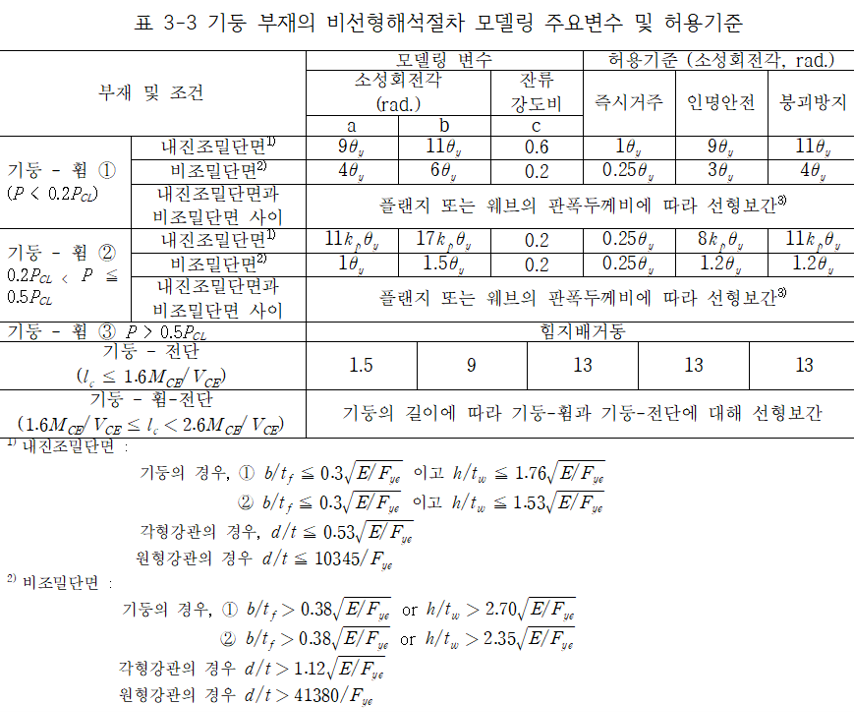
\includegraphics[width=.99\textwidth]{table3-3}
	\end{figure}
\end{frame}


\begin{frame}{3.2 기둥}

	\textbf{3.2.3 기둥의 강도}

3.2.3.2 선형동적절차

\begin{enumerate}
	\item[(1)] 기둥의 예상부재강도 $Q_{CE}$는 휨항복, 횡좌굴, 플랜지국부좌굴, 웨브전단항복의 한계상태를 고려하여 최솟값으로 산정한다. 
	\item[(2)] 웨브전단항복을 제외한 한계상태에 대해 기둥의 휨강도는 $\ulcorner$건축물 강구조 설계기준$\lrcorner$에 제시된 공칭강도 $M_n$에 따라 산정하되, 아래의 사항을 고려한다. 
	\begin{enumerate}[label=\large\protect\textcircled{\small\arabic*}]
		\item 변형지배거동이 예상되는 기둥 부재의 예상휨강도 $M_{CE}$는 강재의 예상재료강도 $F_{ye}$를 적용하여 다음과 같이 산정한다. 
		\[Q_{CE} = M_{CE} = 1.18ZF_{ye}\Big(1 - \frac{P}{P_{ye}}\Big)\leq ZF_{ye}\]
		\item 힘지배거동이 예상되는 기둥 부재의 하한휨강도 $M_{CL}$은 강재의 최소재료강도를 적용하여 산정한다. 
	\end{enumerate}
	\item[(3)] 웨브전단항복의 경우 $M_{CE}$는 $V_{CE}l_b/2$로 산정하며 이 때 $V_{CE}$는 3.7절 링크보요소에 따라 산정한다.  
%		\item[(4)] 보의 전단강도 $V_{CE}$는 $\ulcorner$건축물 강구조 설계기준$\lrcorner$에 따라 산정한다. 불필요해보임
\end{enumerate}
\end{frame}	


\begin{frame}{3.2 기둥}

	\textbf{3.2.3 기둥의 강도}

3.2.3.2 비선형정적 및 동적절차

\begin{enumerate}
	\item[(1)] 비선형정적절차의 경우 표 3-3에 따라 그림 1-1과 같은 비선형 부재력--변형 관계를 결정한다. 기둥의 예상부재강도 $Q_{CE}$는 선형절차와 동일한 값을 사용한다. 
	\item[(2)] 비선형동적절차의 이력거동 모델링은 실험이나 정밀해석을 통해 얻어진 관계를 사용할 수 있으며, 포락곡선으로는 표 3-3에 사용된 모델을 적용할 수 있다. 
\end{enumerate}
\end{frame}	


	\begin{frame}{3.2 기둥}

	\textbf{3.2.4 기둥의 허용기준}

3.2.4.1 일반사항

\begin{enumerate}
	\item[(1)] 압축력과 휨을 동시에 받는 기둥에 작용하는 압축력이 하한압축강도 $P_{CL}$의 50\% 이하인 경우 휨은 변형지배거동으로, 압축은 힘지배거동으로 본다. 
	\item[(2)] 기둥에 작용하는 압축력이 하한압축강도 $P_{CL}$의 50\%를 초과하는 경우, 휨과 압축 모두를 힘지배거동으로 본다. 
	\item[(3)] 기둥에 작용하는 인장은 변형지배거동으로 본다. 인장과 휨이 동시에 작용하는 경우 인장과 휨 모두를 변형지배거동으로 본다. 
\end{enumerate}

	\end{frame}
	
	\begin{frame}{3.2 기둥}

	\textbf{3.2.4 기둥의 허용기준} 
		
3.2.4.2 선형동적절차

\begin{enumerate}
	\item[(1)] 선형동적절차를 위한 기둥의 허용기준은 표 3-4과 같으며, 다음의 사항을 고려한다. 
	\begin{enumerate}[label=\large\protect\textcircled{\small\arabic*}]
		\item 압축력과 휨을 동시에 받는 기둥에 작용하는 압축력이 하한압축강도 $P_{CL}$의 50\% 이하인 경우 \texttt{(휨은 변형지배거동으로, 압축은 힘지배거동으로 보고)} 다음 식에 따라 조합강도를 평가한다.
		\[\begin{dcases}\frac{P_{UF}}{P_{CL}} + \frac{8}{9}\Big[\frac{M_x}{m_x M_{CEx}} + \frac{M_y}{m_y M_{CEy}}\Big] \leq 1.0 & 0.2 \leq \frac{P_{UF}}{P_{CL}} \leq 0.5 \\ \frac{P_{UF}}{2P_{CL}} + \Big[\frac{M_x}{m_x M_{CEx}} + \frac{M_y}{m_y M_{CEy}}\Big] \leq 1.0 & \frac{P_{UF}}{P_{CL}} < 0.2 \end{dcases}\]
	\end{enumerate}	 
\end{enumerate}

	\end{frame}
	
	
		\begin{frame}{3.2 기둥}

	\textbf{3.2.4 기둥의 허용기준} 
		
3.2.4.2 선형동적절차

\begin{enumerate}
	\item[(1)] 선형동적절차를 위한 기둥의 허용기준은 표 3-4과 같으며, 다음의 사항을 고려한다. 
	\begin{enumerate}[label=\large\protect\textcircled{\small\arabic*}]\setcounter{enumii}{1}
		\item 기둥에 작용하는 압축력이 하한압축강도 $P_{CL}$의 50\%를 초과하는 경우 \texttt{(휨과 압축을 힘지배거동으로 보고)} 다음 식에 따라 조합강도를 평가한다.		
		\[\frac{P_{UF}}{2P_{CL}} + \Big[\frac{M_x}{m_x M_{CEx}} + \frac{M_y}{m_y M_{CEy}}\Big] \leq 1.0\]
		\item 기둥에 작용하는 인장은 변형지배거동으로 본다. 인장과 휨이 동시에 작용하는 경우 \texttt{(인장과 휨 모두 변형지배거동으로 보고)} 다음 식에 의해 기둥을 평가한다. 
		\[\frac{T}{m_t T_{CE}} + \Big[\frac{M_x}{m_x M_{CEx}} + \frac{M_y}{m_y M_{CEy}}\Big] \leq 1.0\]
	\end{enumerate}	 
\end{enumerate}

	\end{frame}

\begin{frame}
	\begin{figure}
		\centering
		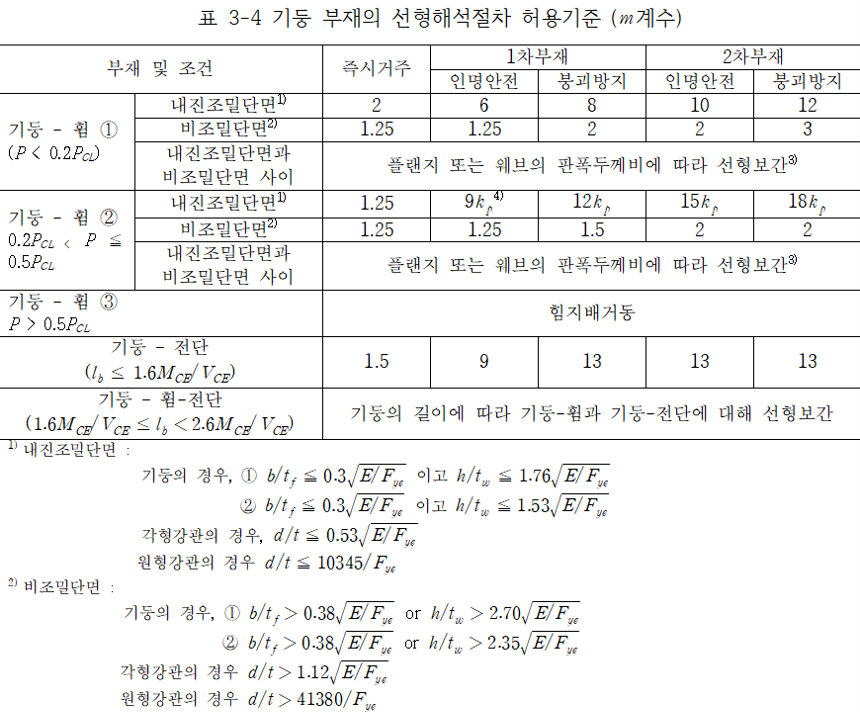
\includegraphics[width=.99\textwidth]{table3-4}
	\end{figure}
\end{frame}

	\begin{frame}{3.2 기둥}
	
3.2.4.2 비선형 정적 및 동적절차	

기둥 부재의 소성회전변형 허용기준은 표 3-3을 따른다. 

	\begin{figure}
		\centering
		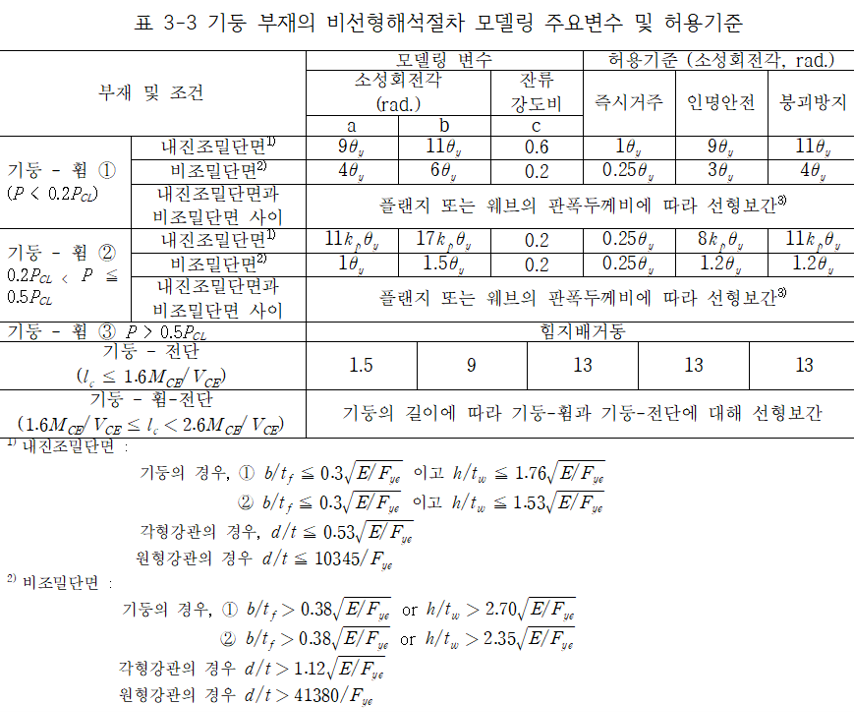
\includegraphics[width=.7\textwidth]{table3-3}
	\end{figure}
\end{frame}

